\documentclass[./main.tex]{subfiles}

\begin{document}

\section{Misassemblies in noisy assemblies}

Originaly publish in: \url{https://blog.pierre.marijon.fr/misassemblies-in-noisy-assemblies/}

Author: Pierre Marijon

\subsection{Introduction}

I think that all the people who have ever done a genome assembly one day
say: "Ok my assembly is cool, but now how I can be sure that it's the
best and it doesn't contain a lot of errors ?"

We have many technics to evaluate the quality of assemblies (it isn't a
complete review, sorry):

\begin{itemize}
\item with only assembly information:
  \begin{itemize}
  \item with \href{https://doi.org/10.1089/cmb.2017.0013}{N50 family metrics}
  \item by analyzing reads remapping against assembly \href{http://amos.sourceforge.net/wiki/index.php/Amosvalidate}{AMOSValidate}, \href{https://www.sanger.ac.uk/science/tools/reapr}{REAPR}, \href{https://github.com/vezzi/FRC_align}{FRCbam}, \href{https://github.com/broadinstitute/pilon/wiki}{Pilon}, \href{https://www.cbcb.umd.edu/software/valet}{VALET}
  \item by computing the probability of the reads given the assembly (\href{https://doi.org/10.1093/bioinformatics/bts723}{ALE}, \href{https://doi.org/10.1186/gb-2013-14-1-r8}{CGAL}, \href{https://doi.org/10.1186/1756-0500-6-334}{LAP})
  \end{itemize}
\item by using external information:
  \begin{itemize}
  \item count the number of core genes present in an assembly, \href{https://busco.ezlab.org/}{BUSCO}
  \item transcriptome information, \href{https://doi.org/10.1186/gb-2009-10-4-r42}{for example, \emph{Bos taurus} genome validation}
  \item synteny information \href{https://doi.org/10.1186/s12859-018-2026-4}{Lui et al}
  \item map assembly against a near reference genome, \href{https://doi.org/10.1093/bioinformatics/btt086}{quast} or \href{https://bmcgenomics.biomedcentral.com/articles/10.1186/s12864-019-6070-x}{dnAQET}
  \end{itemize}
\end{itemize}

Note that for the last bullet point, if you are using quast with a
reference genome you already have, by definition, a reference genome. So
why perform an assembly?

The main reason to perform reference-assisted evaluation is when testing
different assembly pipelines on the same read data set. To evaluate a
new assembly pipeline, one also has to test different sets of
parameters, and evaluate the impact of adding or changing the tools that
are part of the pipeline.

Quast is a very useful tool and now it integrates many other assembly
evaluating tools (BUSCO,
\href{http://exon.gatech.edu/GeneMark/}{GeneMark},
\href{https://doi.org/10.1093/bioinformatics/bth315}{GlimmerHMM},
\href{https://github.com/tseemann/barrnap}{barnap})

Recently, with Rayan Chikhi and Jean-Stéphane Varré, we published a
\href{https://www.biorxiv.org/content/10.1101/674036v2}{preprint} about
\href{https://github.com/natir/yacrd/}{yacrd} and
\href{https://github.com/natir/fpa}{fpa}, two new standalone tools.
These tools can be included in assembly pipelines to remove very bad
reads regions, and filter out low-quality overlaps. We evaluated the
effect of these tools on some pipelines
(\href{https://github.com/lh3/miniasm}{miniasm} and
\href{https://github.com/ruanjue/wtdbg2}{redbean}). Using quast, we
compared the results with the assembly quality of different pipelines.

We sent this paper to a journal, and one of the reviewers said something
along the lines of: "quast isn't a good tool to evaluate
high-consensus-error assemblies, the number of misassemblies was
probably over evaluated."\\
And it's probably true.

Miniasm and redbean perform assemblies without read correction steps
(and without consensus step for miniasm). The low quality of a contig
sequence is a real problem: quast could confuse a misaligned low-quality
region with a misassembly.

In this blog post, I want to answer the following questions:

\begin{enumerate}
\def\labelenumi{\arabic{enumi}.}
\item how to run quast on long-read uncorrected misassemblies
\item is the quast misassemblies count a good proxy to evaluate / compare assemblies?
\item can we find better metrics than just the number of misassemblies?
\end{enumerate}

If you have no time to read all these long and technical details you can
go directly to the \protect\hyperlink{take-home-message}{TL;DR}.

In this post I will talk about quast and not dnAQET, which has just been
released, but dnAQET uses the same method (mapping the assembly against
the reference) and the same misassembly definition as quast. It seems to
me that what I am going to say about quast also applies to dnAQET. But
go read the dnAQET publication, there are lots of super interesting
ideas in it.

\subsection{Datasets, assembly pipelines, analysis pipelines; versions
and parameters}

For our tests we are going to use two Nanopore datasets and one Pacbio
dataset.

\begin{itemize}
\item Reads:
  \begin{itemize}
  \item \href{https://www.ebi.ac.uk/ena/data/view/SRX3676783}{Oxford nanopore D melanogaster} 63x coverage
  \item \href{http://s3.amazonaws.com/nanopore-human-wgs/chr1.sorted.bam}{Oxford nanopore H sapiens chr1} 29x
  \item \href{http://datasets.pacb.com.s3.amazonaws.com/2014/c_elegans/list.html}{Pacbio RS P6-C4 C elegans} 80x
  \end{itemize}
\item References:
  \begin{itemize}
  \item \href{https://www.ncbi.nlm.nih.gov/assembly/GCF_000001215.4}{D.
    melanogaster} 143.7 Mb
  \item \href{ftp://ftp.ensembl.org/pub/release-95/fasta/caenorhabditis_elegans/dna/Caenorhabditis_elegans.WBcel235.dna.toplevel.fa.gz}{C.
    elegans} 100.2 Mb
  \item \href{ftp://ftp.ensembl.org/pub/release-95/fasta/homo_sapiens/dna/Homo_sapiens.GRCh38.dna.chromosome.1.fa.gz}{H. sapiens chr1} 248.9 Mb
  \end{itemize}
\end{itemize}

To perform assembly we use minimap2 (version 2.16-r922) and miniasm
(version 0.3-r179) with recommended preset for each sequencing
technology (\texttt{ava-ont} and \texttt{ava-pb}).

We use \href{https://github.com/lbcb-sci/racon}{racon} (v1.4.3) for
polishing. For mapping reads against assembly we use minimap2, with
recommended preset for each sequencing technology.

We use quast version v5.0.2.

All dotplots were produced by
\href{http://dgenies.toulouse.inra.fr/}{D-Genies}.

\subsection{Quast misassemblies definition}

What are quast misassemblies? Do we have different misassembly types?
How are they defined?

Quast defines three types of misassemblies: \textbf{relocation},
\textbf{translocation} and \textbf{inversion}.

\subsubsection{Relocation}

A relocation can occur based on signal from two mappings of the same
contig against the same chromosome (cf Figure \ref{relocation_def}). We have two cases:

\begin{itemize}
\item either the two mappings are separated by an unmapped region (case \textbf{A})
\item or they map on the same chromosome with a shared mapping area (case \textbf{B})
\end{itemize}

\begin{figure}[ht]
    \centering
    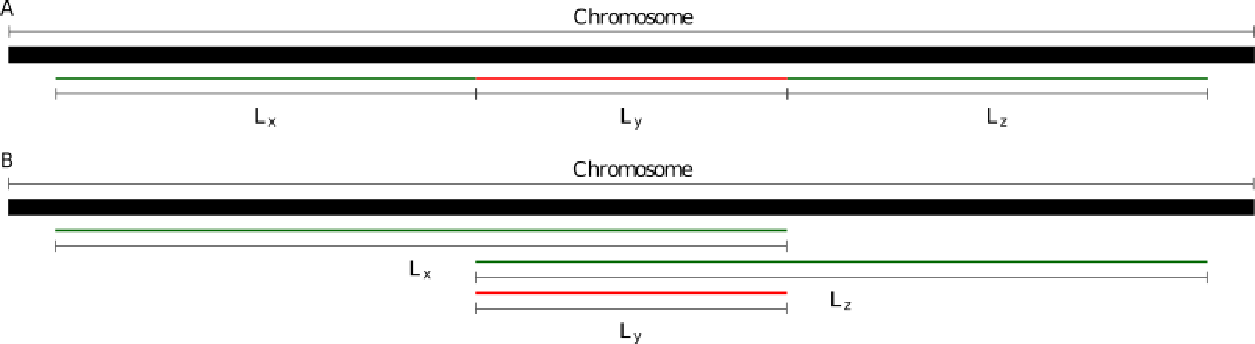
\includegraphics[width=\textwidth]{paper/misassemblies-in-noisy-assemblies/relocation_def.pdf}
    \caption{A schematic representation of a relocation}
    \label{relocation_def}
\end{figure}

A misassembly is said to occur when $L_x$ and $L_z$ \textgreater{}
1kbp (this value can't be changed, it seems) and when $L_y$
\textgreater{} \texttt{extensive-mis-size} (1kbp by default).

Let's call $L_y$ the length of the relocation.

\begin{itemize}
\item The relocation length is positive when the assembly missed a part of the reference (case \textbf{A})
\item Negative when the assembly includes a duplicated region (case \textbf{B}).
\end{itemize}

In both cases, this is an assembly error.

\begin{figure}[ht]
    \centering
    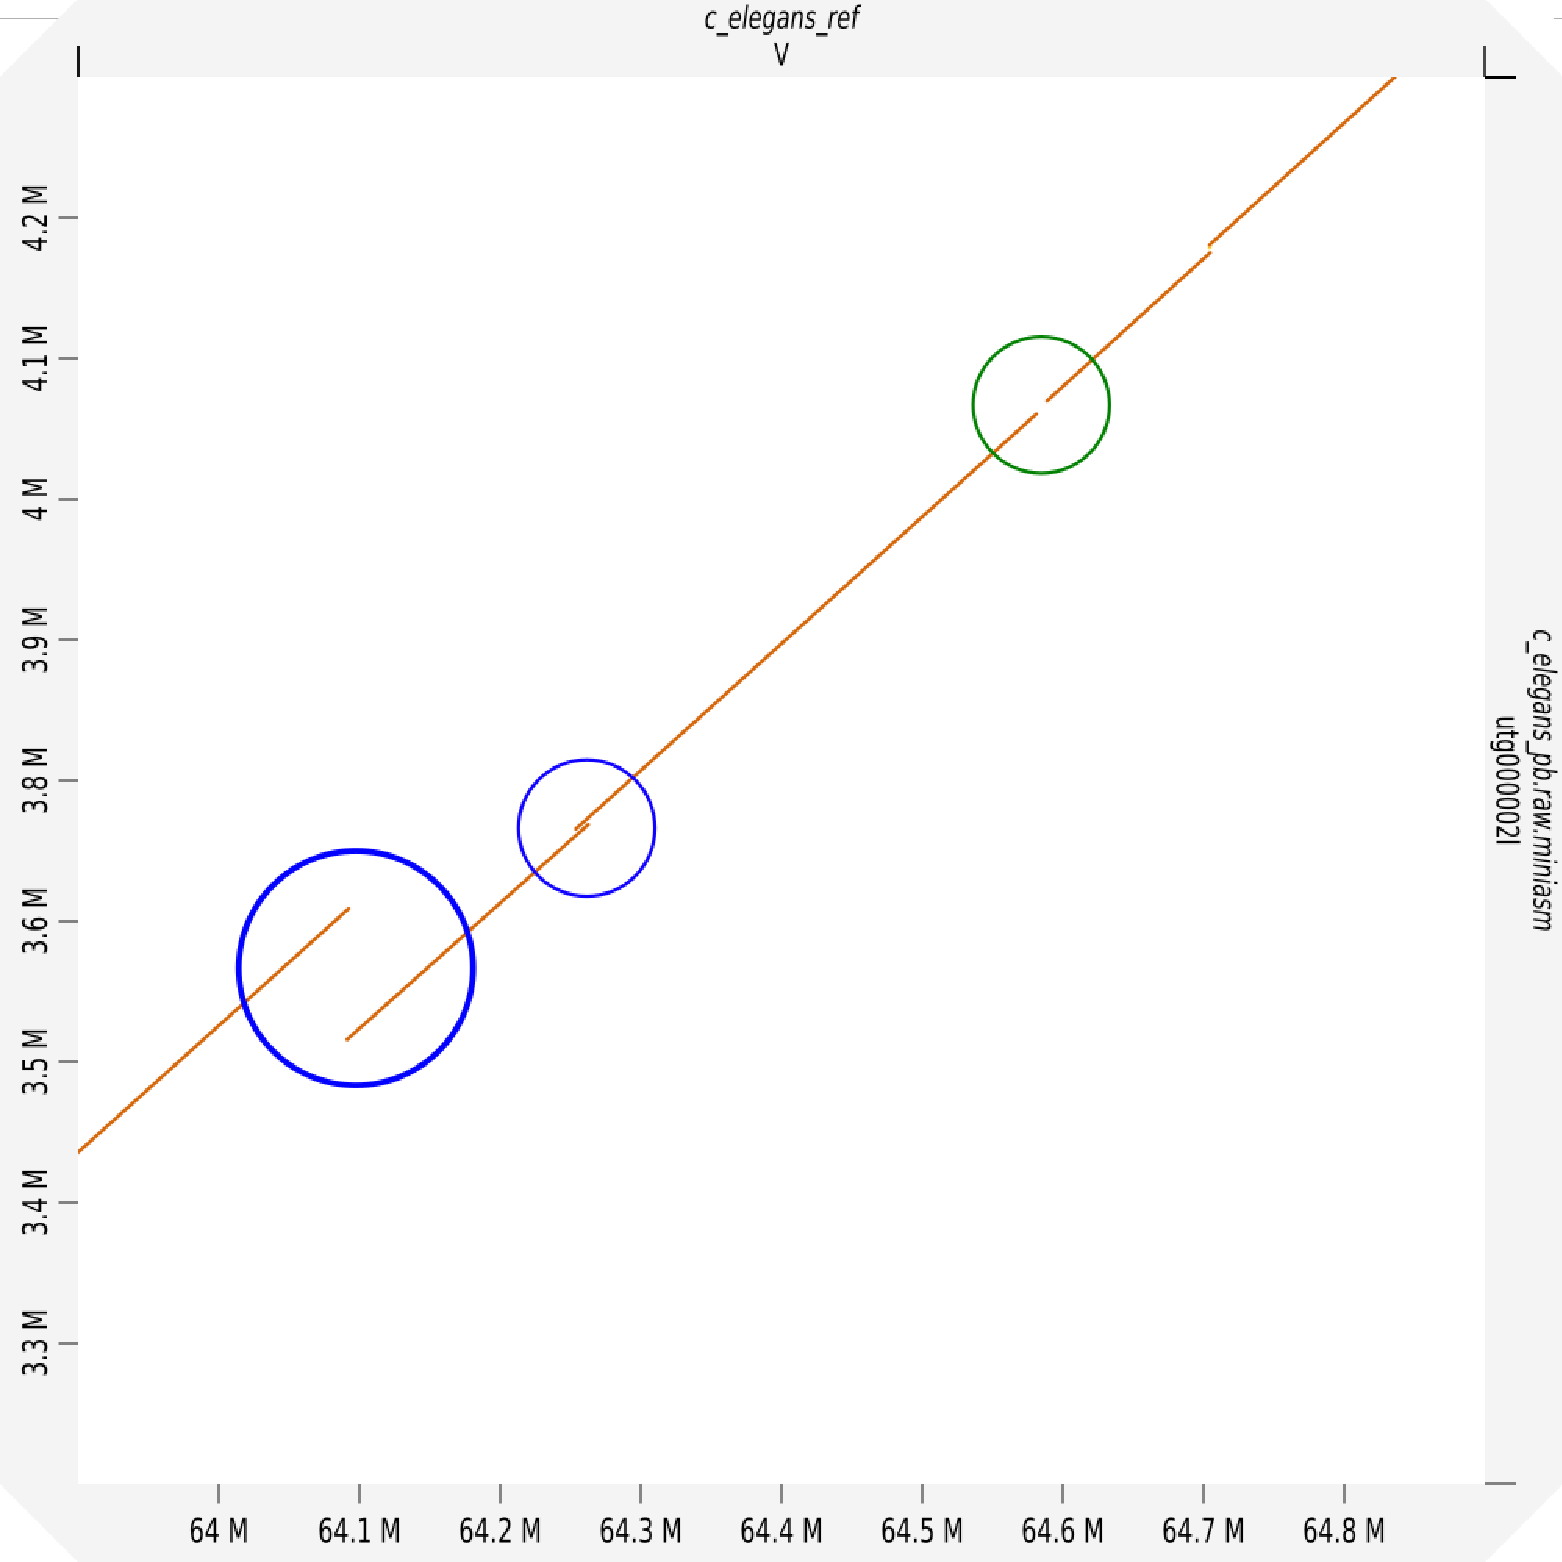
\includegraphics[width=0.5\textwidth]{paper/misassemblies-in-noisy-assemblies/relocation_dotplot_exemple.pdf}
    \caption{Thrid relocation observe in dotplot a long reads assembly against reference of \textit{C. elegans}}
    \label{relocation_exp}
\end{figure}

In dotplot present in Figure \label{relocation_exp} of contigs ctg000002L for our \emph{C. elegans}
miniasm assembly against the chromosome V of the reference. We can see
two relocation events of type \textbf{B} circled in blue and one
relocation event of type \textbf{A} (green). I have no idea on how to
explain the other problem on the top right.

\subsubsection{Translocations}

A translocation occurs when a contig has mapped on more than one reference chromosome (cf Figure \ref{translocation_def}).
\begin{figure}[ht]
    \centering
    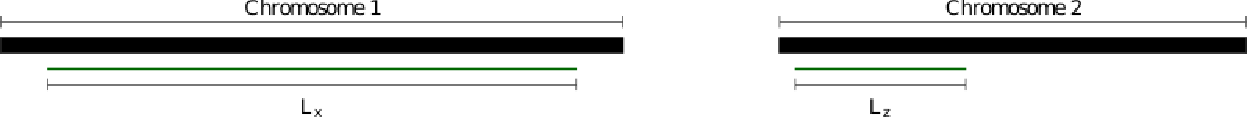
\includegraphics[width=\textwidth]{paper/misassemblies-in-noisy-assemblies/translocation_def.pdf}
    \caption{A schematic representation of a translocation}
    \label{translocation_def}
\end{figure}

It's easy to spot this kind of misassemblies on a dotplot because of the
multi-chromosome match.

\begin{figure}[ht]
    \centering
    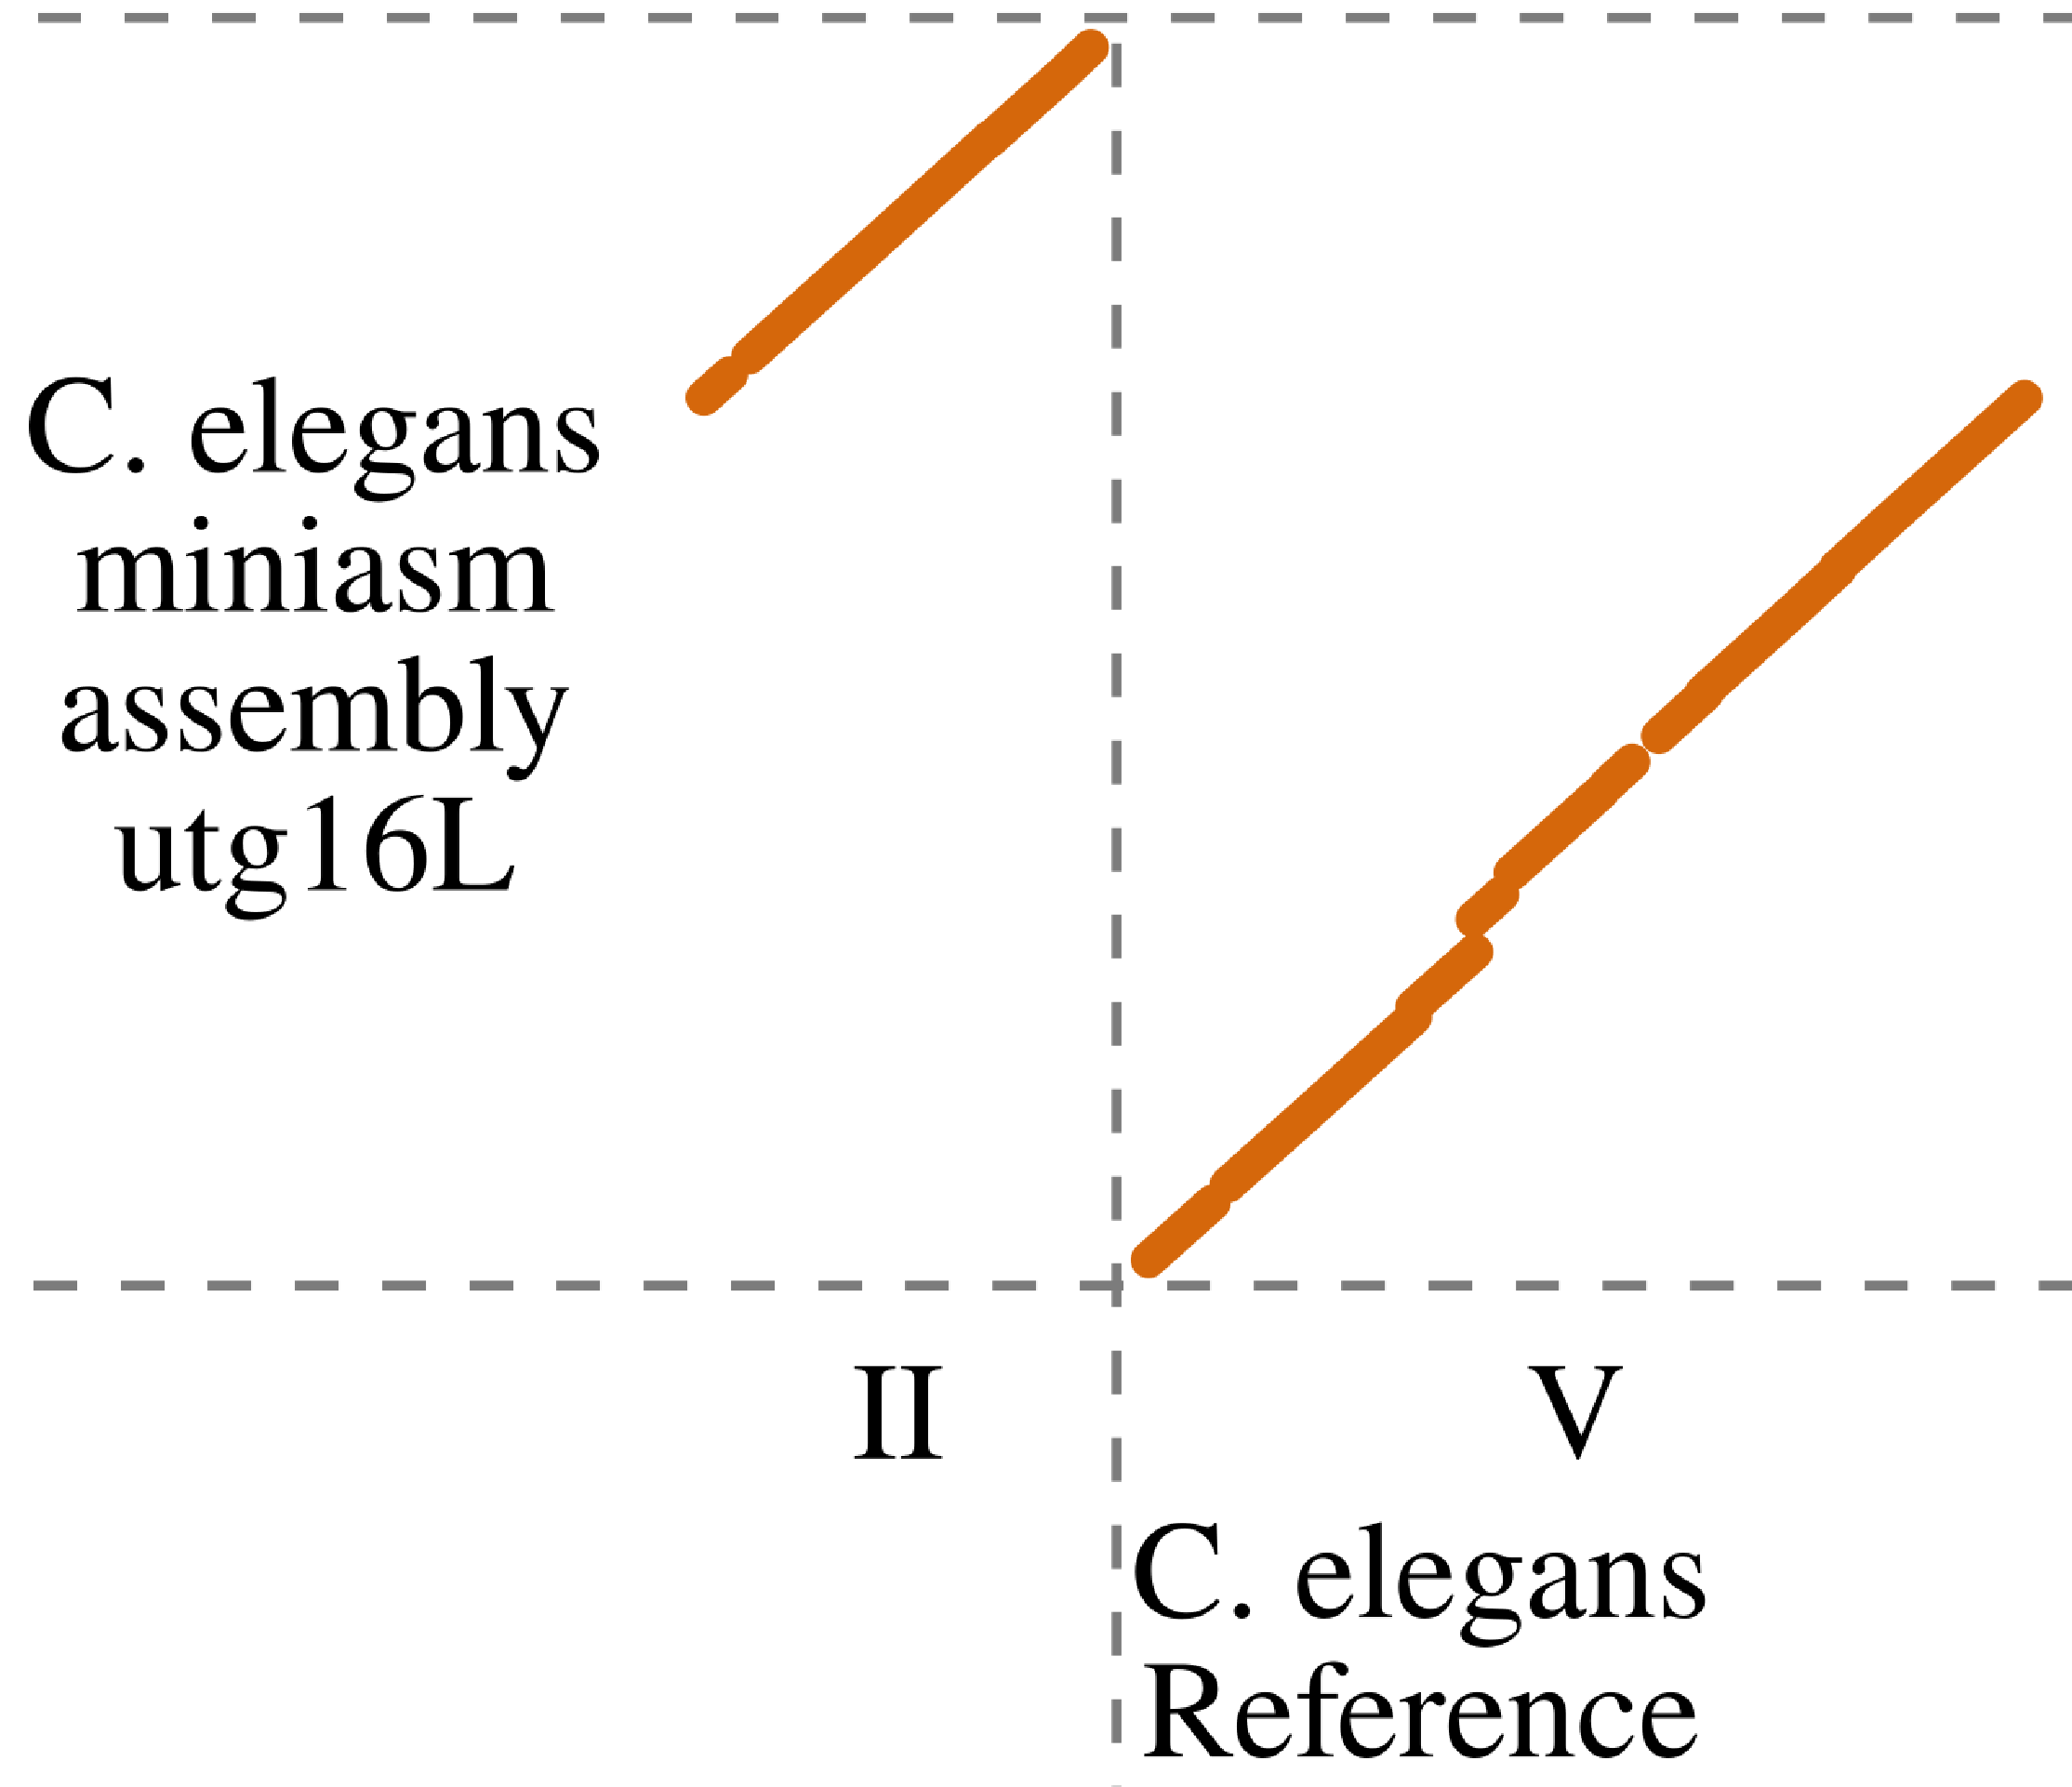
\includegraphics[width=0.5\textwidth]{paper/misassemblies-in-noisy-assemblies/translocation_dotplot_exemple.pdf}
    \caption{A translocation in a dotplot.}
    \label{translocation_exp}
\end{figure}

In Figure \ref{translocation_exp}, two parts of contig 'utg16L' from our \emph{C. elegans} miniasm assembly, map respectively on chromosomes II and V of the reference. This contig contains a translocation without any doubt.

\subsubsection{Inversions}

An inversion occurs when a contig has two consecutive mappings on the
same chromosome but in different strands (cf Figure \ref{inversion_def}).

\begin{figure}[ht]
    \centering
    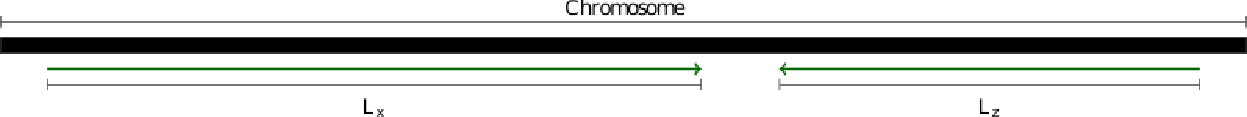
\includegraphics[width=\textwidth]{paper/misassemblies-in-noisy-assemblies/inversion_def.pdf}
    \caption{A schematic representation of a inversion}
    \label{inversion_def}
\end{figure}

The dotplot present in Figure \ref{inversion_exp} shows an inversion between a reference genome and a
miniasm assembly of \emph{C. elegans}.

\begin{figure}[ht]
    \centering
    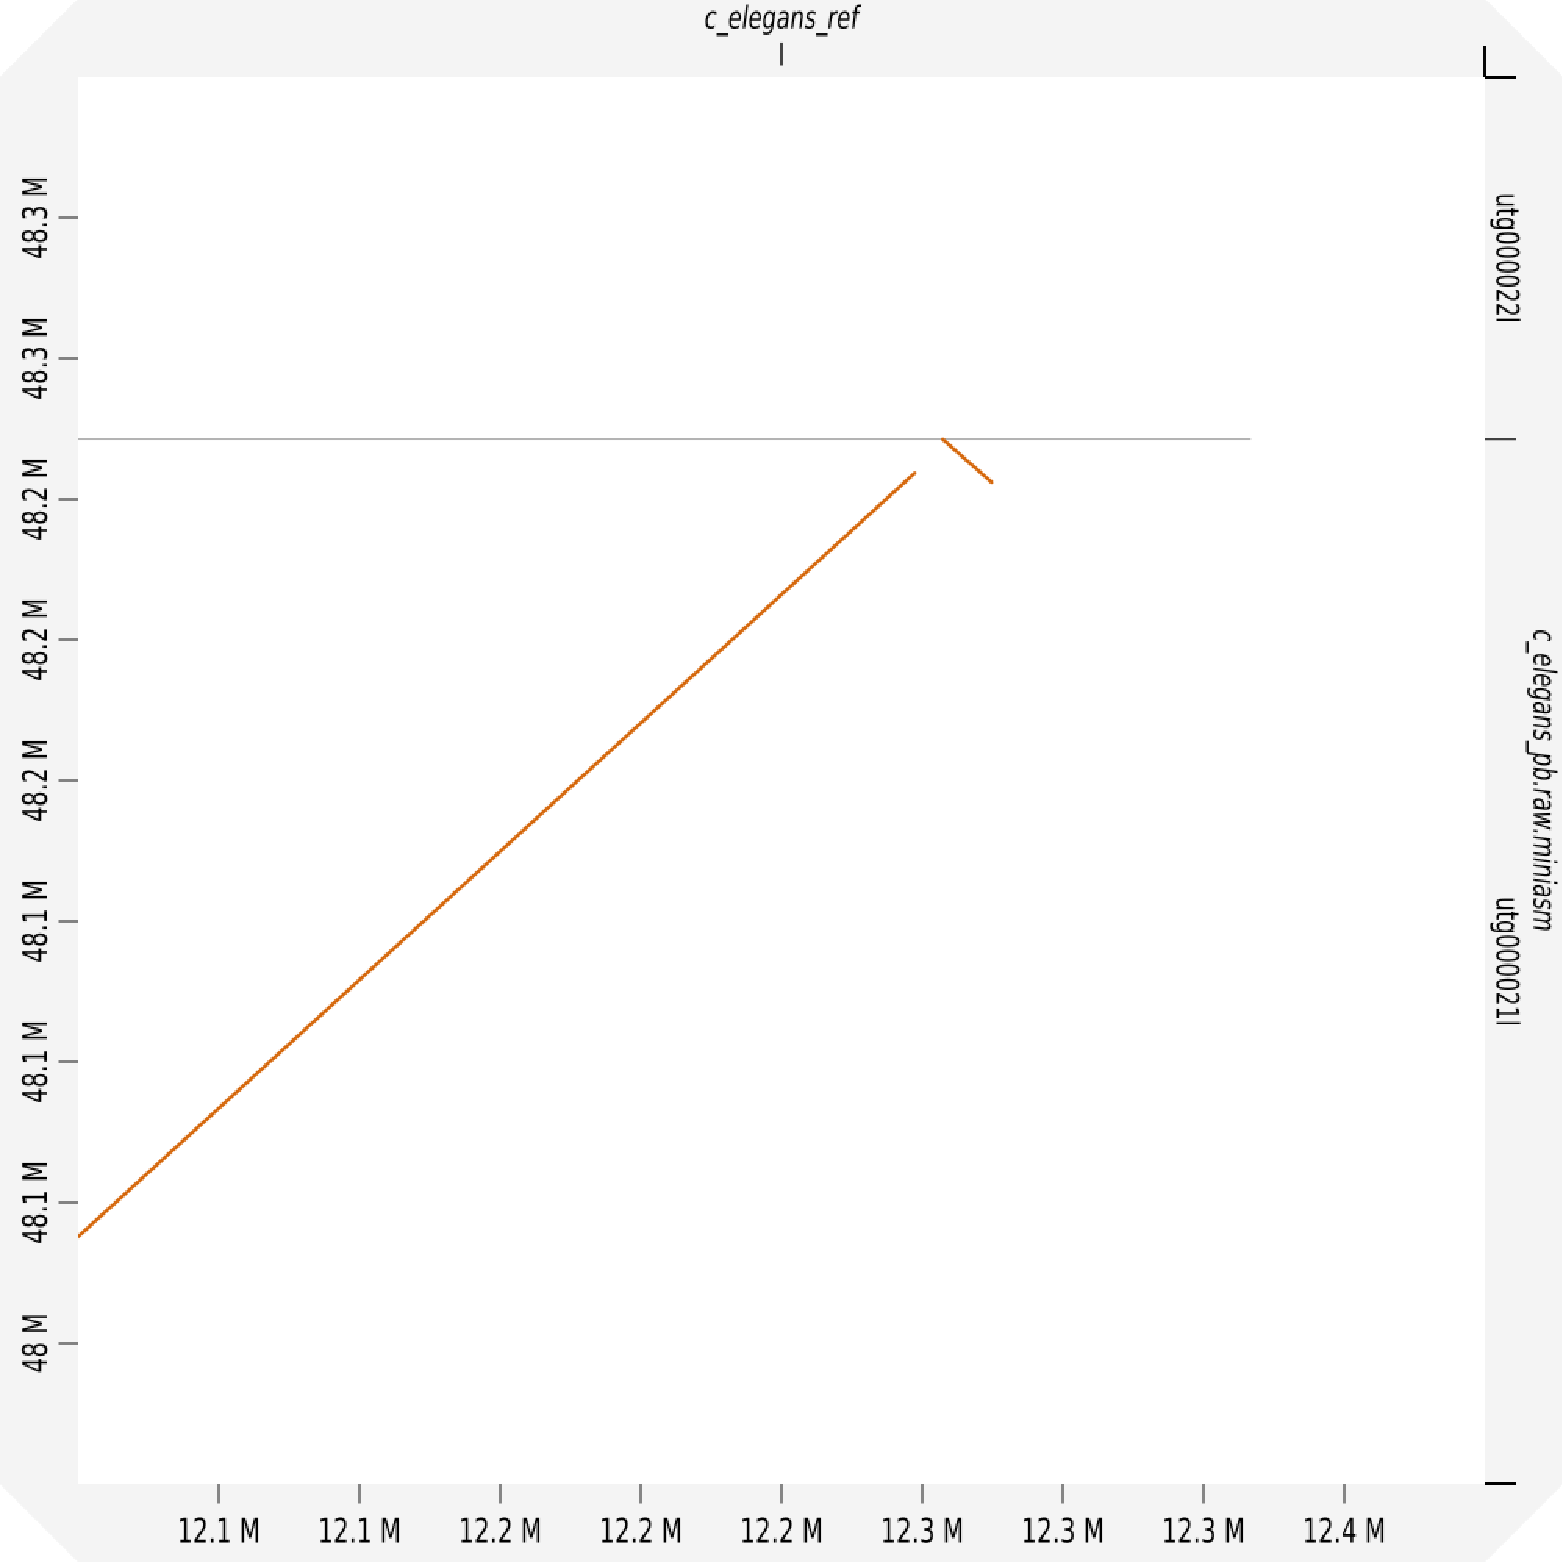
\includegraphics[width=0.5\textwidth]{paper/misassemblies-in-noisy-assemblies/inversion_dotplot_exemple.pdf}
    \caption{The contig utg0000021L maps on chromosome I, but it contains a small inversion at its end.}
    \label{inversion_exp}
\end{figure}

\subsubsection{Important point}

For more details on quast misassembly definitions, you can read this
section \href{http://quast.bioinf.spbau.ru/manual.html\#misassemblies}{3.1.1} and section \href{http://quast.bioinf.spbau.ru/manual.html\#sec3.1.2}{3.1.2} of the quast manual.

Quast bases its misassemblies analysis on the alignmnt of contigs
against a reference. To perform alignment, recent versions of quast use
\href{https://github.com/lh3/minimap2}{minimap2}, with preset
\texttt{-x\ asm5} by default, or \texttt{-x\ asm20}
\href{https://github.com/ablab/quast/blob/b040cc9140c7630eea95f94cdda3b825cf4a22c3/quast_libs/ca_utils/align_contigs.py\#L65}{when
min-identity is lower than 90\%}. After that, alignments with identity
lower than \texttt{min-identity} are filtered out by quast (95\%
identity by default, but can be set to as low as 80\%).

\texttt{min-identity} is a very important parameter. To consider a
contig as misassembled, quast must have a minimum of two mappings for
this contig. If the second mapping has an identity under the
\texttt{min-identity} threshold, quast can't observe the misassembly.
But even more, if a contig has three successive mappings, and assume
also that the mapping in the middle has lower identity than the
\texttt{min-identity} threshold, and the remaining gap between the two
other mappings is larger than \texttt{extensize-mis-size}, then quast
sees this as a misassembly, where in fact it isn't.

\textbf{Parameters \texttt{min-identity} and \texttt{extensize-mis-size}
have an important impact on misassemblies detection. So, what is the
effect of changes in of these two parameters on the number of
misassemblies found by quast?}

\subsection{Effect of min-identity}

\subsubsection{Low min-identity is required for uncorrected assembly}

Quast only uses mappings with alignment identity higher than
\texttt{min-identity}. So, what could be a good value for this parameter
for long-read uncorrected assembly?

The file
\texttt{contigs\_reports/minimap\_output/\{output-name\}.coords},
generated by quast, in the fourth column contains the alignment identity
\%. For each dataset, we extracted this value and plot it in an
histogram (cf \ref{mapping_identity}).

\begin{figure}[ht]
    \centering
    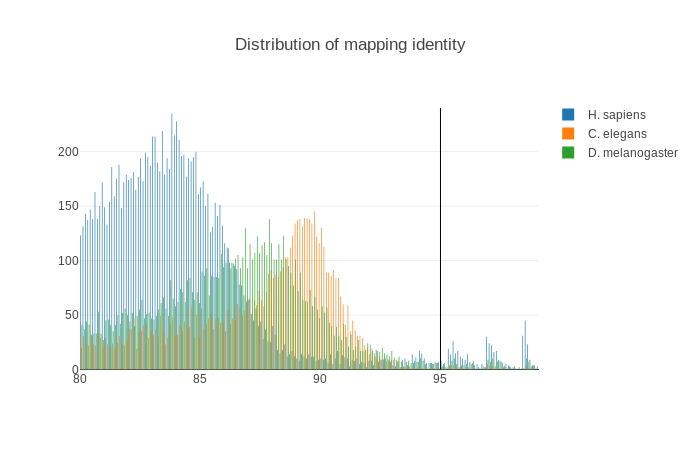
\includegraphics[width=\textwidth]{paper/misassemblies-in-noisy-assemblies/misassemblies_mapping_identity_distribution.png}
    \caption{Horizontal axis: identity percentage bins, vertical axis: number of mappings in each bin.}
    \label{mapping_identity}
\end{figure}

The black line marks quast default identity value threshold, we can see
a majority of alignments are under this threshold for an uncorrected
dataset. So, setting parameter \texttt{min-identity\ 80} seems
necessary.

\subsubsection{Effect on a polished assembly}

To test the effect of correction on misassemblies count, we ran racon 3
times on \emph{C. elegans} (the one with the best reference) dataset.

On the non-corrected assembly, quast makes use of 7049 mappings; for the
corrected assembly, 30931 mappings (increasing ratio 4.38).

\begin{figure}[ht]
    \centering
    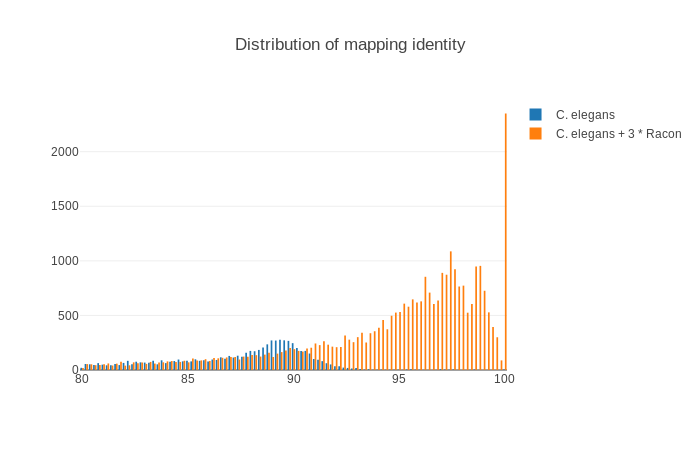
\includegraphics[width=\textwidth]{paper/misassemblies-in-noisy-assemblies/misassemblies_mapping_identity_distribution_racon.png}
    \caption{Horizontal axis: identity percentage bins, vertical axis: number of mappings in each bin.}
    \label{mapping_identity_racon}
\end{figure}

We can observe in Figure \ref{mapping_identity_racon} an increase in alignment identity due to racon
(unsurprisingly). Contrary to the uncorrected assembly, a majority of
the mappings now have 95\% or more identity.

To have an insight on the effect of \texttt{min-identity} on
unpolished/polished assemblies, we run quast with default parameters and
changing only \texttt{min-identity} (still the \emph{C. elegans}
dataset).

\begin{table}[ht]
    \centering
    \begin{tabular}{l|rrr}
    racon & no & yes & yes \\
    min-identity & 80 & 80 & 95 \\ \hline 
    relocation & 1131 & 886 & 635 \\
    translocation & 200 & 259 & 170 \\
    inversion & 65 & 68 & 75 \\
    total & 1396 & 1213 & 880 \\
    \end{tabular}
    \caption{This table shows the number of different types of misassemblies, whether we run racon on the assembly or not and according to the value of the threshold \texttt{min-identity}}
    \label{tab:my_label}
\end{table}

With \texttt{min-identity\ 80} the number of relocations and
translocations is increased compared to the default value of
\texttt{min-identity}. If quast has only one alignment of a contig, it
cannot find misassemblies. By reducing the \texttt{min-identity} we
increased the number of alignments and mechanically increased the number
of detected misassemblies.

We think that some of these misassemblies aren't real misassemblies. But
if we use the same \texttt{min-identity} value for all assemblies that
we want to compare, we can hope that the number of 'false' misassemblies
will be similar.

\textbf{For uncorrected long-read assemblies, we recommend to use a
lower-than-default QUAST identity threshold parameter (80 \%)}

\subsection{Effect of extensive-mis-size on misassemblies count}

We observed that the \texttt{min-identity} parameter has a very
important impact on the number of misassemblies for uncorrected
long-read assemblies (-\textgreater{} need to set it to 80 \%.) Now we
want to observe what is the impact of another parameter:
\texttt{extensive-mis-size}, which is a length threshold for the
detection of relocation-type misassemblies.

We launch quast with different value for parameter
\texttt{extensive-mis-size}: 1.000, 2.000, 3.000, 4.000, 5.000, 6.000,
7.000, 8.000, 9.000, 10.000, 20.000, 30.000, 40.000, 50.000 (in base
pairs). The parameter \texttt{min-identity} was set to 80 \%.

\begin{figure}
    \centering
    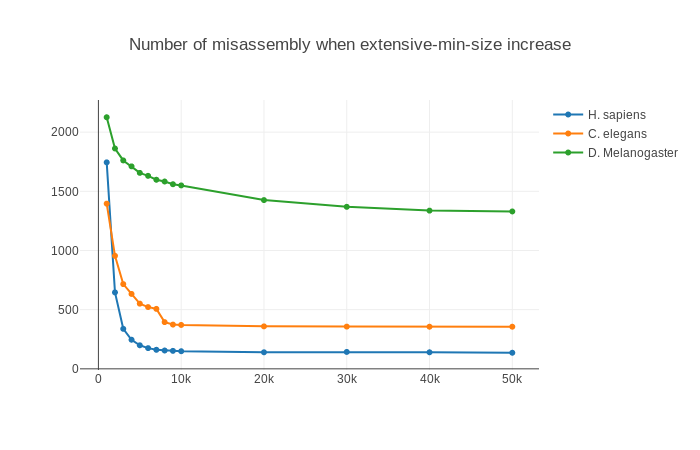
\includegraphics[width=\textwidth]{paper/misassemblies-in-noisy-assemblies/misassemblies_x_extensive_mis_size.png}
    \caption{In the horizontal axis, we have the \texttt{extensive-mis-size} value.
In the vertical axis we have the number of misassemblies.}
    \label{misassemblies_x_all}
\end{figure}

The Figure \ref{misassemblies_x_all} shows the evolution of the number of misassemblies in
function of the \texttt{extensive-mis-size} value. After 10.000 base
pairs, the number of misassemblies becomes quite stable.

This graph shows two regimes: with \texttt{extensive-mis-size} lower
than 10.000 bp, it detects quite a lot of misassemblies. With
\texttt{extensive-mis-size} higher than 10.000 bp, it detects less of
them. \textbf{Yet we know that quast detects three type of misassemblies
(relocations, translocations, inversions). Only relocation should be
affected by \texttt{extensive-mis-size} parameter, but let's verify this
assumption.}

\subsubsection{Effect of parameter extensive-mis-size on the detection
of each misassembly type}

Quast defines three types of misassemblies \textbf{relocation},
\textbf{translocation} and \textbf{inversion}. Previously we observed
the total number of misassemblies. Now we break down by group of
misassemblies (cf Figure \ref{misassemblies_x_types}).

\begin{figure}[ht]
    \centering
    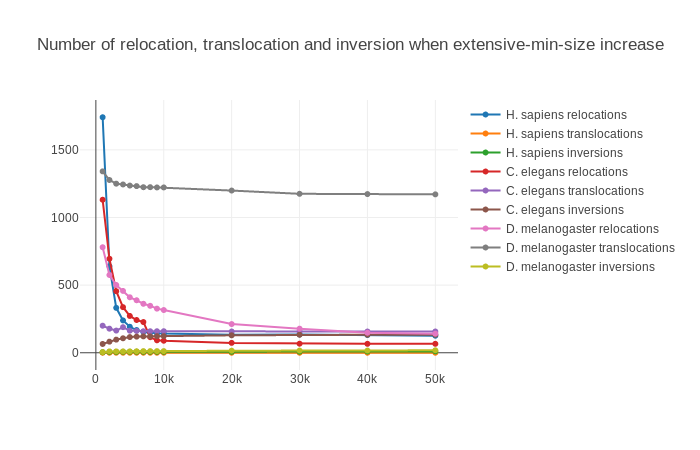
\includegraphics[width=\textwidth]{paper/misassemblies-in-noisy-assemblies/misassemblies_x_extensive_mis_size_type.png}
    \caption{In the horizontal axis, we have the \texttt{extensive-mis-size} value.
In the vertical axis, we have the number of misassemblies.}
    \label{misassemblies_x_types}
\end{figure}

The \emph{H. sapiens} dataset doesn't have any translocation because the
reference is composed of only one chromosome. The majority of
misassemblies are relocations, but when we increase the parameter
\texttt{extensive-mis-size} the number of inversions also increases.

\emph{D. melanogaster} reference contains many small contigs. This can
explain the high number of translocations. Relocations and
translocations drop at the same time.

For \emph{C. elegans} the number of translocations was quite stable, the
number of relocations drops down rapidly and the inversions has only a
little increase.

I can't explain why translocations and inversions numbers change with a
different value of \texttt{extensive-mis-size}. By reading quast
documentation and code I didn't understand the influence of this
parameter on this group of misassemblies.

\textbf{Relocation misassemblies are the most common type of
misassemblies. We can impute the reduction of misassemblies, when
\texttt{extensive-mis-size} grows, to a reduction of relocations.}

\subsubsection{Relocations lengths distribution}

We see previously for our assemblies that a majority of misassemblies
were relocations. We are now focused on this type of misassemblies. For
each relocation we can attach a length, this length is the length of
incongruence between assembly and reference genome. It's equal to
$L_y$.

The file
\texttt{\{quast\_output\}/contigs\_reports/all\_alignements\_\{assembly\_file\_name\}.tsv}
contains information about mapping and misassemblies. For other
information on how quast stores mapping and misassemblies information,
read \href{http://quast.bioinf.spbau.ru/manual.html\#sec7}{quast faq}.

\begin{figure}
    \centering
    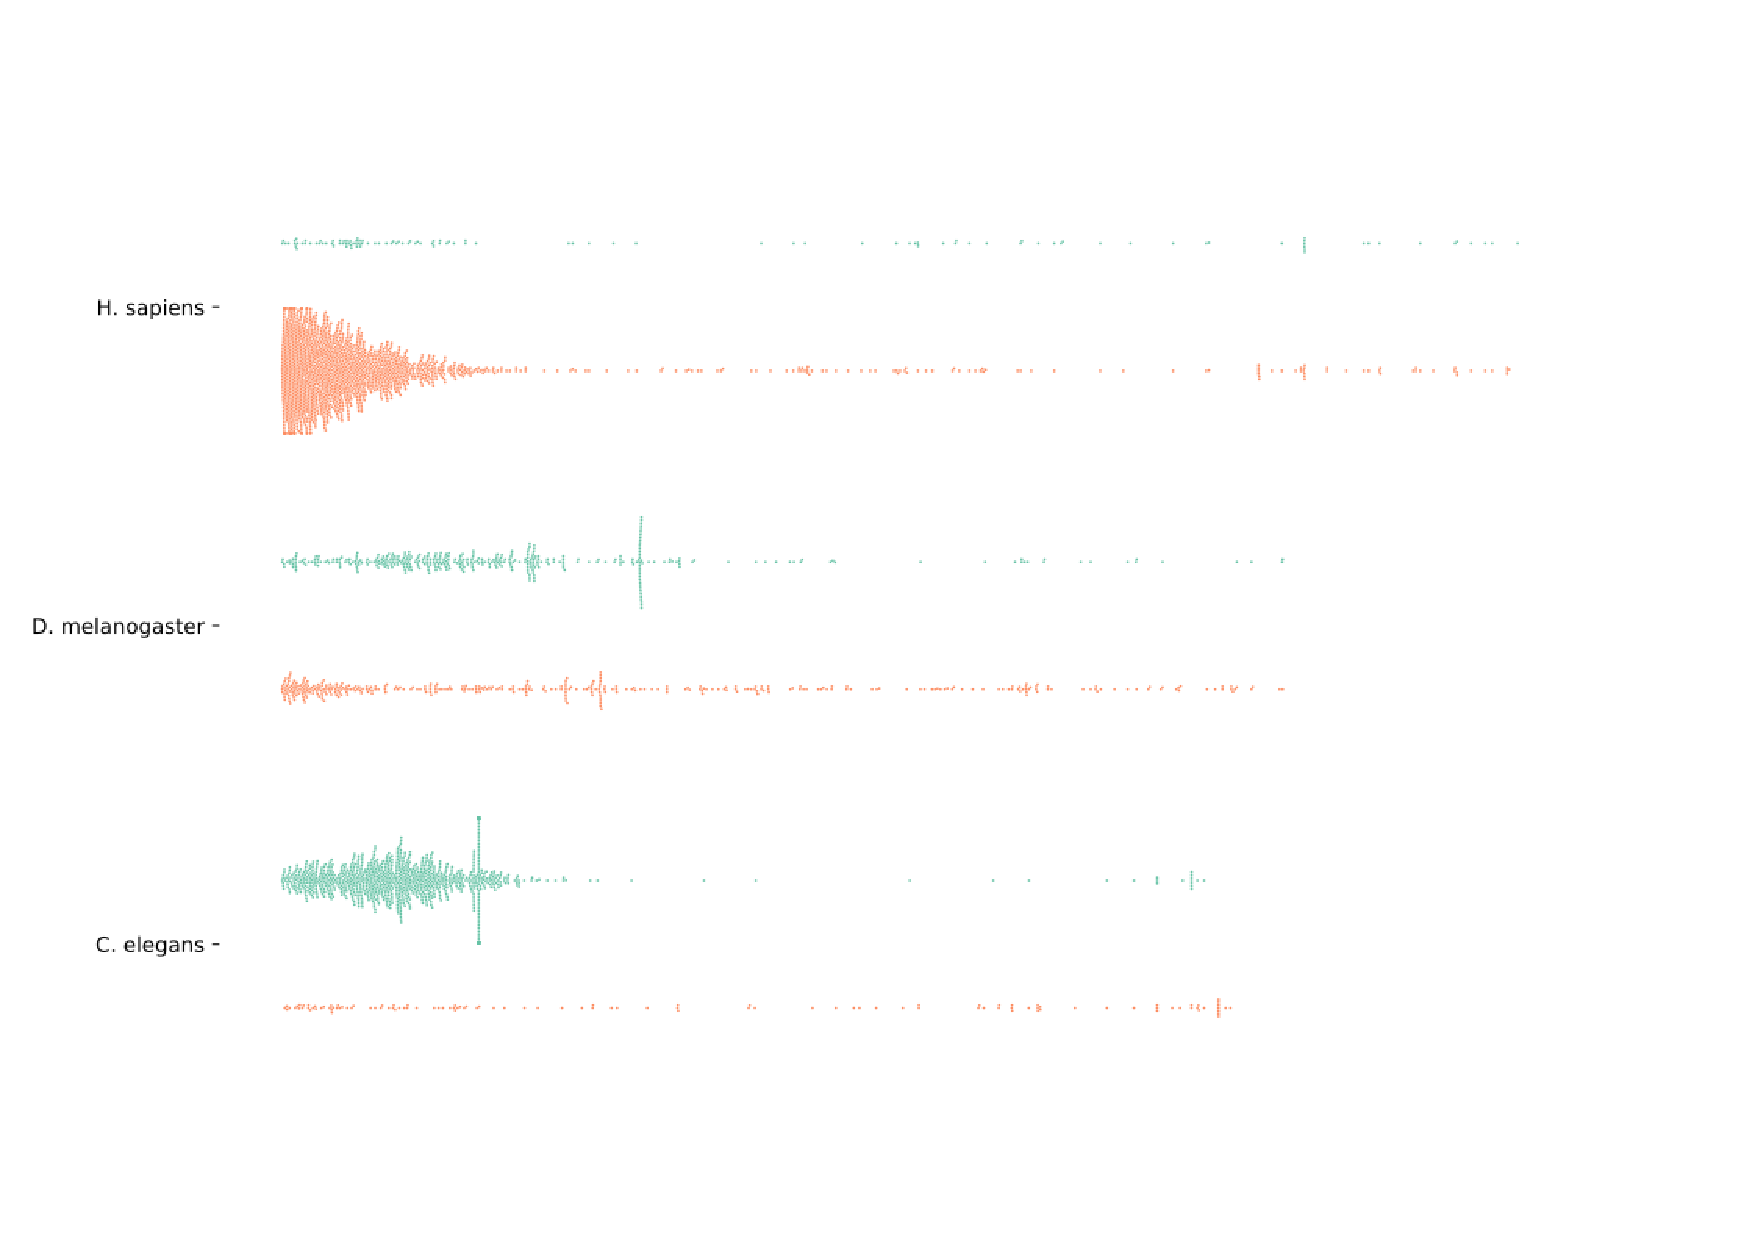
\includegraphics[width=\textwidth]{paper/misassemblies-in-noisy-assemblies/relocation_length.pdf}   
    \caption{In the vertial axis, we have the log length of each relocation. Each raw is a species. Orange points are for negative (\textless{}0 bp) relocations, green points for positive relocations.}
    \label{swarmplot}
\end{figure}

The Figure \ref{swarmplot} shows a swarm plot of log of length associated to
recombination. It's the size of the gap between mappings flankings a
misassembly. If the length is positive, the assembly misses part of the
reference (green point). If the length is negative, the assembly
duplicates a part of the reference (orange point).
\href{relocation_length.py}{Source code},
\href{relocation_length.csv}{data} is available.

For \emph{H. sapiens} a majority of relocations were positive and short
(between 1000 and 5000 bases), with some very large relocations. For
\emph{C. elegans} it's different, the majority of relocations are
negative and the largest relocation was shorter than in \emph{H.
sapiens}. For \emph{D. melanogaster} the size of relocations was more
spread out; the majority of relocations aren't short. This is confirmed
by the look of the curve seen in the previous part, when
\texttt{extensize-mis-size} is increased, the number of relocations
decreases less quickly than for the other datasets.

\textbf{With this representation, we can analyze the differences in
relocations between assemblies, in terms of their numbers and more
importantly the distributions of their lengths.}

\subsection{Conclusion}

If you work with quast to evaluate an assembly made with miniasm, you
need to set \texttt{min-identity} parameter to 80 \%. It would be nice
to have a lower minimum value, maybe 70\%, but the quast code would have
to be modified. And such a low identity is required only for a miniasm
assemblies; for tools with a better consensus step (redbean for
exemple), 80 \% seems sufficient.

Translocations and inversions constitute a minority within
misassemblies, yet when they are detected it's clear that they are
'true' misassemblies. I would be very surprised to see a translocation
or inversion created by a mapping error, itself generated by error(s) in
an uncorrected long-reads assembly. We can thus trust the count of
translocations and inversions.

For relocations, the situation is different. They constitute the
majority of misassemblies in our cases, and some of them are \emph{true}
some of them are \emph{false}. Checking all misassemblies manualy is
impossible, and finding a good \texttt{extensive-mis-size} value seems
very hard for me. The easiest thing we can do is compare the series of
lengths associated to relocations, as shown in this blogpost I used a
swarmplot; I think statisticians could find better tools.

\subsection{Take home message}

You can use quast to compare uncorrected long-reads assemblies but:

\begin{itemize}
\item run quast with \texttt{--min-identity 80}
\item rely on translocations and inversions counts
\item for relocations, compare distributions of lengths associated to each assembly
\end{itemize}

\subsection{Acknowledgements}

For the creation of this very effective and useful tool all Quast
contributors.

For their help in writing this blogpost:

\begin{itemize}
\item Rayan Chikhi
\item Jean-Stéphane Varré
\item Yoann Dufresne
\item Antoine Limasset
\item Matthieu Falce
\item Kevin Gueuti
\end{itemize}

\end{document}